`%%%%%%
%
% $Autor: Manoj Selvaraju $
% $Datum: 2024-01-05 11:15:45Z $
% $Pfad: githubtemplate/Template/report/rename.tex $
% $Version: 4620 $
%
%
% !TeX encoding = utf8
% !TeX root = Rename
% !TeX TXS-program:bibliography = txs:///bibtex
%
%%%%%%

\chapter{Arduino Command Line Interface (CLI)}

Arduino Command Line Interface (CLI) is an all-in-one solution that provides Boards/Library Managers, sketch builder, board detection, uploader, and many other tools needed to use any Arduino compatible board and platform from command line or machine interfaces.
In addition to being a standalone tool, Arduino CLI is the heart of all official Arduino development software (Arduino IDE, Arduino Web Editor). This means that all functionalities provided by the development environment are also available here. This can be used under Windows, MacOS and Linux \cite{ArduinoCLIpro:2024}. Development using the command line interpreter makes it possible to carry out quality assurance measures in a targeted manner if batch files are used consistently. This means that the configuration of the development environment can be saved and repeated in a traceable manner.


The source code can be used freely, but a license must be requested from the company for commercial use \cite{ArduinoCLIGit:2024}. Detailed documentation is provided. \cite{ArduinoCLIDoc:2024}

The development of the Command Line Interface (CLI) focuses on three aspects.
\begin{enumerate}
  \item On the one hand, the interface can be embedded within familiar development tools, making it easier to work with platforms like Edge Impulse for machine learning at the edge.
  \item Secondly, it enables the integration of development into the Continuous Development and Continuous Integration processes. It thus enables the automation of typical software development activities.
  \item Furthermore, it now enables simplified communication with edge computers, for example with a Raspberry PI.
\end{enumerate}

\section {Installing and using the CLI}
As \ac{cli} is constantly being further developed, the current version must first be downloaded from the GitHub project \href{https://arduino.github.io/arduino-cli/0.36/installation/}{Arduino-cli-0.36-installation}, see \cite{ArduinoCLIGit:2024}. The version used here is 0.36.0 \cite{ArduinoCLIversion:2024}

\bigskip

After successfully downloading the file \FILE{arduino-cli\_1.0.4\_Windows\_64bit.zip}, the folder contents can be extracted to a self-defined storage path \PATH{C:/Program Files/Arduino CLI}. The packed file contains the license terms and the executable file \FILE{arduino-cli.exe}. 

In order to use the function of the command line interpreter in different paths, the path \PATH{C:/Program Files/Arduino CLI} to the storage location of the file \FILE{arduino-cli.exe} should be added to the system variable \SHELL{PATH} as shown in the below Figure ~\ref{Path}. The interface can then be used by entering \SHELL{arduino-cli} in the command line.

\begin{figure}
	\begin{center}
		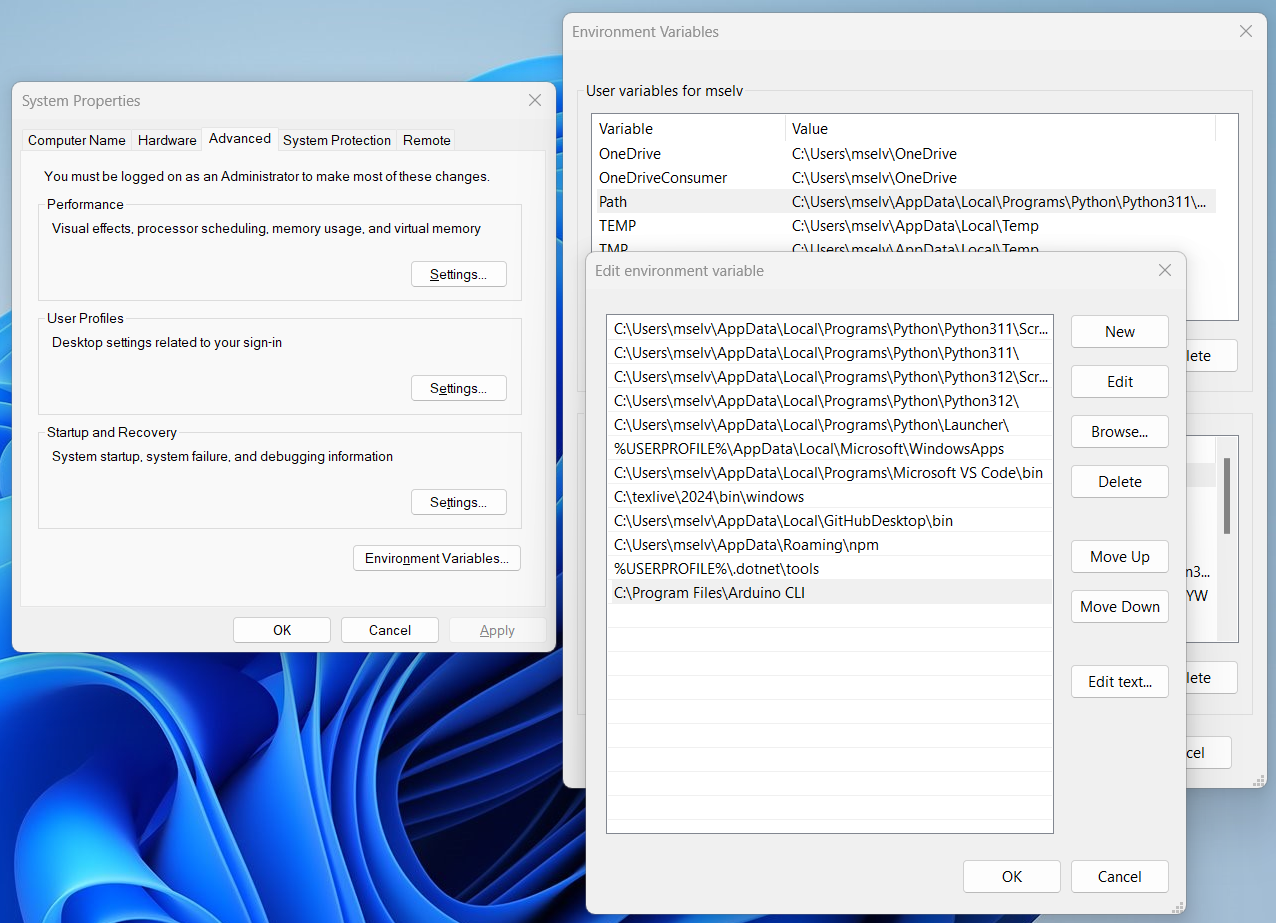
\includegraphics[width=0.7\linewidth]{Images/ArduinoCLI/ArduinocliPATH.png}
		\caption{Adding arduino-cli.exe file storage location to PATH system variable}
		\label{Path}
	\end{center}
\end{figure}


After the installation is complete, \SHELL{arduino-cli board list} can be entered in the command prompt. The connected device is displayed as Arduino Portenta H7 with port number and type, as shown in Figure ~\ref{Installation}.  

\begin{figure}
	\begin{center}
		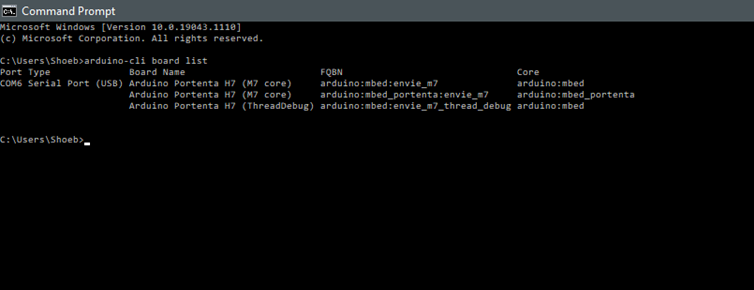
\includegraphics[width=0.7\linewidth]{Images/ArduinoCLI/CLIInstallation.png}
		\caption{Installation of Arduino CLI}
		\label{Installation}
	\end{center}
\end{figure}

\subsection{Arduino CLI License}
Arduino CLI is licensed under the GPL 3.0 license. The software is open-source and licensed under the GNU General Public License (GPL) version 3, which means it is free to use, modify, and distribute it as long as you comply with the GPL terms. While there is typically a license file included in the download to explain the legal terms, but its presence is not required for the software to function. Buying a commercial license is mandatory if you want to modify or otherwise use the software for commercial activities involving the Arduino software without disclosing the source code of your own applications. \cite{ArduinoCLIGit:2024}


\section{Configuration of the Arduino CLI}
So that CLI can find the Arduino installation, it helps to create a configuration file for CLI. This configuration file is defined in a format \SHELL{YAML}. To create a basic configuration file, CLI can be used in which a command line
\SHELL{arduino-cli config init}
is entered. This command creates a new file \FILE{arduino-cli.yaml} in the following path \PATH{C:/Users/mselv/AppData/\\Local/Arduino15/arduino-cli.yaml}. All necessary parameters are declared there. The default settings of the configuration file are shown in the listing ~\ref{lst:yaml-config}. 

% Default settings of the configuration file
%\lstinputlisting[language=Python, firstline=1, %lastline=27]{../Code/Arduino/ArduinoCLI/yaml.py}

\begin{code}
\begin{center}
\begin{lstlisting}[language=yaml,caption={Default settings of the configuration file},label={lst:yaml-config}]
		board_manager:
		additional_urls: []
		build_cache:
		compilations_before_purge: 10
		ttl: 720h0m0s
		daemon:
		port: "50051"
		directories:
		data: C:\Users\mselv\AppData\Local\Arduino15
		downloads: C:\Users\mselv\AppData\Local\Arduino15\staging
		user: C:\Users\mselv\OneDrive\Documents\Arduino
		library:
		enable_unsafe_install:  false
		logging:
		file: ""
		format: text
		level: info
		metrics:
		addr: :9090
		enabled:  true
		output:
		no_color:  false
		sketch:
		always_export_binaries:  false
		updater:
		enable_notification:  true
	\end{lstlisting}
\end{center}
\end{code}

The following parameters usually need to be changed:
\begin{itemize}
	\item \FILE{sketchbook\_path}: Directory of the Arduino sketchbook. All libraries and hardware definitions are installed here.
	\item \FILE{Arduino\_data}: Installation location of the Arduino board and the library manager. In most cases, this should not need to be changed.
\end{itemize}
The other options can generally remain at their default values.


\subsection{Configuration keys}

Configuration keys refer to the parameters or settings stored in the configuration file \FILE{arduino-cli.yaml}. These keys determine various aspects of how the Arduino CLI operates. \cite{ArduinoCLIConfig:2024}

\begin{itemize}
	\item \SHELL{board\_manager}
	\begin{itemize}
		\item \SHELL{additional\_urls} - the URLs to any additional Boards Manager package index files needed for your boards platforms.
	\end{itemize}
	\item \SHELL{daemon} - options related to running Arduino CLI as a gRPC server.
	\begin{itemize}
		\item \SHELL{port} - TCP port used for gRPC client connections.
	\end{itemize}
	\item \SHELL{directories} - directories used by Arduino CLI.
	\begin{itemize}
		\item \SHELL{data} - directory used to store Boards/Library Manager index files and Boards Manager platform installations.
		\item \SHELL{downloads} - directory used to stage downloaded archives during Boards/Library Manager installations.
		\item \SHELL{user} - the equivalent of the Arduino IDE's "sketchbook" directory. Library Manager installations are made to the libraries subdirectory of the user directory.
		\item \SHELL{builtin.libraries} - the libraries in this directory will be available to all platforms without the need for the user to install them, but with the lowest priority over other installed libraries with the same name, it's the equivalent of the Arduino IDE's bundled libraries directory.
		\item \SHELL{builtin.tools} - it's a list of directories of tools that will be available to all platforms without the need for the user to install them, it's the equivalent of the Arduino IDE 1.x bundled tools directory.
	\end{itemize}
	    \item \SHELL{library} - configuration options relating to Arduino libraries.
	\begin{itemize}
		\item \SHELL{enable\_unsafe\_install} - set to true to enable the use of the --git-url and --zip-file flags with arduino-cli lib install. These are considered "unsafe" installation methods because they allow installing files that have not passed through the Library Manager submission process.
	\end{itemize}
	\item \SHELL{locale} - the language used by Arduino CLI to communicate to the user, the parameter is the language identifier in the standard POSIX format <language>[\_<TERRITORY>[.<encoding>]] (for example it or it\_IT, or it\_IT.UTF-8).
	\item \SHELL{logging} - configuration options for Arduino CLI's logs.
	\begin{itemize}
		\item \SHELL{file} - path to the file where logs will be written.
		\item \SHELL{format} - output format for the logs. Allowed values are text or json.
		\item \SHELL{level} - messages with this level and above will be logged. Valid levels are: trace, debug, info, warn, error, fatal, panic.
	\end{itemize}
	\item \SHELL{metrics} - settings related to the collection of data used for continued improvement of Arduino CLI.
	\begin{itemize}
		\item \SHELL{addr} - TCP port used for metrics communication.
		\item \SHELL{enabled} - controls the use of metrics.
	\end{itemize}
	\item \SHELL{output} - settings related to text output.
	\begin{itemize}
		\item \SHELL{no\_color} - ANSI color escape codes are added by default to the output. Set to true to disable colored text output.
	\end{itemize}
	\item \SHELL{sketch} - configuration options relating to Arduino sketches.
	\begin{itemize}
		\item \SHELL{always\_export\_binaries} - set to true to make arduino-cli compile always save binaries to the sketch folder. This is the equivalent of using the --export-binaries flag.
	\end{itemize}
	\item \SHELL{updater} - configuration options related to Arduino CLI updates
	\begin{itemize}
		\item \SHELL{enable\_notification} - set to false to disable notifications of new Arduino CLI releases, defaults to true
	\end{itemize}
	\item \SHELL{build\_cache} - configuration options related to the compilation cache
	\begin{itemize}
		\item \SHELL{compilations\_before\_purge} - interval, in number of compilations, at which the cache is purged, defaults to 10. When 0 the cache is never purged.
		\item \SHELL{ttl} - cache expiration time of build folders. If the cache is hit by a compilation the corresponding build files lifetime is renewed. The value format must be a valid input for time.ParseDuration(), defaults to 720h (30 days).
	\end{itemize}
		\item \SHELL{network} - configuration options related to the network connection.
	\begin{itemize}
		\item \SHELL{proxy} - URL of the proxy server.
	\end{itemize}
\end{itemize}

\subsection{Configuration methods}
Arduino CLI may be configured in three ways:
\begin{enumerate}
	\item Command line flags
	\item Environment variables
	\item Configuration file
\end{enumerate}

If a configuration option is configured by multiple methods, the value set by the method highest on the above list overwrites the ones below it.

If a configuration option is not set, Arduino CLI uses a default value.

\SHELL{arduino-cli config dump} displays the current configuration values. Detailed documentation is provided \cite{ArduinoCLIConfig:2024}

\subsubsection{Command line flags}
Configuration file of Arduino CLI can be modified using Command line flags. \cite{ArduinoCLIConfig:2024}
\begin{itemize}
	\item Example:
	Setting an additional Boards Manager URL using the \SHELL{--additional-urls} command line flag:
	\newline
	\PYTHON{arduino-cli core update-index --additional-urls}
	\newline
	\PYTHON{https://downloads.arduino.cc/packages/package\_staging\_index.json}
\end{itemize}

\subsubsection{Environment variables}
All configuration options can be set via environment variables. The variable names start with \SHELL{ARDUINO}, followed by the configuration key names, with each component separated by \SHELL{\_}. For example, the \SHELL{ARDUINO\_DIRECTORIES\_USER} environment variable sets the directories.user configuration option.
\\On Linux or macOS, you can use the \SHELL{export} command to set environment variables. On Windows command, you can use the \SHELL{set} command. \cite{ArduinoCLIConfig:2024}
\begin{itemize}
	\item Example:
Setting an additional Boards Manager URL using the \SHELL{ARDUINO\_BOARD\_MANAGER\_ADDITIONAL\_URLS} environment variable:
\newline
\PYTHON{set ARDUINO\_BOARD\_MANAGER\_ADDITIONAL\_URLS=}
\newline
\PYTHON{https://downloads.arduino.cc/packages/package\_staging\_index.json}

	\begin{itemize}
		\item The export or set command should be run in terminal session. It sets the environment variable for the duration of that terminal session.
		\item If the terminal is closed, the environment variable will be unset. To make the variable persistent across terminal sessions, we should add the export or set command to shell's configuration file (e.g., .bashrc, .zshrc, or .profile).
	\end{itemize}
\end{itemize}

\subsubsection{Configuration file}
\SHELL{arduino-cli config init} creates or updates a configuration file with the current configuration settings.
This allows saving the options set by command line flags or environment variables. \cite{ArduinoCLIConfig:2024}
\begin{itemize}
	\item Example:
\PYTHON{arduino-cli config init --additional-urls}
\newline
\PYTHON{https://downloads.arduino.cc/packages/package\_staging\_index.json}
\\The configuration file must be named \FILE{arduino-cli}, with the appropriate file extension for the file's format.
\end{itemize}

Refer the listing ~\ref{lst:yaml-config-upd}, for the updation of the configuration file using \SHELL{arduino-cli config init}

\begin{code}
	\begin{center}
		\begin{lstlisting}[language=yaml,caption={Updated settings of the configuration file},label={lst:yaml-config-upd}]
			board_manager:
			additional_urls: 
			     : https://downloads.arduino.cc/packages/package_staging_index.json
			build_cache:
			compilations_before_purge: 10
			ttl: 720h0m0s
			daemon:
			port: "50051"
			directories:
			data: C:\Users\mselv\AppData\Local\Arduino15
			downloads: C:\Users\mselv\AppData\Local\Arduino15\staging
			user: C:\Users\mselv\OneDrive\Documents\Arduino
			library:
			enable_unsafe_install:  false
			logging:
			file: ""
			format: text
			level: info
			metrics:
			addr: :9090
			enabled:  true
			output:
			no_color:  false
			sketch:
			always_export_binaries:  false
			updater:
			enable_notification:  true
		\end{lstlisting}
	\end{center}
\end{code}

\section{Overview of functions}
The file \FILE{README.md} in the GitHub repository "Arduino CLI" contains an excellent overview of the functions and possibilities \cite{ArduinoCLIGit:2024}
The following functions are available \cite{ArduinoCLIversion:2024}:

\begin{itemize}
	\item \SHELL{arduino-cli}
	\item \SHELL{board}
	\begin{itemize}
		\item \SHELL{board attach}
		\item \SHELL{board details}
		\item \SHELL{board list}
		\item \SHELL{board listall}
		\item \SHELL{board search}
	\end{itemize}
	\item \SHELL{burn-bootloader}
	\item \SHELL{cache}
	\item \SHELL{cache clean}
	\item \SHELL{compile}
	\item \SHELL{completion}
	\item \SHELL{config}
	\begin{itemize}
		\item \SHELL{config dump}
		\item \SHELL{config init}
		\item \SHELL{config add}
		\item \SHELL{config delete}
		\item \SHELL{config remove}
		\item \SHELL{config set}
	\end{itemize}
	\item \SHELL{core}
	\begin{itemize}
		\item \SHELL{core download}
		\item \SHELL{core install}
		\item \SHELL{core list}
		\item \SHELL{core search}
		\item \SHELL{core uninstall}
		\item \SHELL{core update-index}
		\item \SHELL{core upgrade}
	\end{itemize}
	\item \SHELL{daemon}
	\item \SHELL{debug}
	\item \SHELL{lib}
	\begin{itemize}
		\item \SHELL{lib deps}
		\item \SHELL{lib download}
		\item \SHELL{lib examples}
		\item \SHELL{lib install}
		\item \SHELL{lib list}
		\item \SHELL{lib search}
		\item \SHELL{lib uninstall}
		\item \SHELL{lib update-index}
		\item \SHELL{lib upgrade}
	\end{itemize}
	\item \SHELL{monitor}
	\item \SHELL{outdated}
	\item \SHELL{sketch}
	\begin{itemize}
		\item \SHELL{sketch archive}
		\item \SHELL{sketch new}
	\end{itemize}
	\item \SHELL{update}
	\item \SHELL{upgrade}
	\item \SHELL{upload}
	\item \SHELL{version}
\end{itemize}

\subsection{Basic functions}

The functions required to load a finished sketch onto an Arduino are defined as basic functions. Communication with a connected Arduino is implemented later using the serial monitor.

\bigskip
The first basic function is the board list command. This can be used to display all Arduino boards connected to the PC with additional information - such as the port used or the core of the board. This information is necessary for using the correct board.
The core list and core install commands are also required. The already installed cores can be listed with the core list command. If the core specified under board list is not installed, it can be added with the core install command.
The third basic function is the lib command with the lib list and lib install extensions. The lib list command can be used to check which libraries are already installed on the system. If an additional library is required for a sketch, it can be installed with the lib install command.

The preparations for compiling and uploading a sketch can be made with these basic functions. By executing the compile command, a sketch is compiled into code that can be read by a selected board. A compiled sketch is then uploaded to a board using the upload command. The port of the board known from the board list command is specified as the destination for the upload. The basic functions are summarized  in Table \ref{CLITableBasicFunction}

\begin{center}
	\begin{table}[h]
		\captionabove{List of Basic Functions}
		\begin{tabular}{c|c|l}
			No. & BasicFunction & Description \\ \hline
			1 & \SHELL{board list} & List the connected Arduinos with additional information \\
			2 & \SHELL{core list}/\SHELL{install} & List and install cores \\
			3 & \SHELL{lib list}/{install} & Listing and installing libraries \\
			4 & \SHELL{compile} & Compiling a sketch for a specific board \\
			5 & \SHELL{upload} & Uploading a sketch to an Arduino \\
		\end{tabular}
		\label{CLITableBasicFunction}
	\end{table}
\end{center}


\subsection{Command reference}

Arduino Command Line Interface includes the following syntax format. \cite{ArduinoCLIversion:2024}
 \PYTHON{arduino-cli <command> [flags]}
	\begin{itemize}
		\item \textbf{<command>} - represents the CLI commands to be executed.
		\item \textbf{flags} - represents optional command-line arguments that can modify the behavior of the command. These flags provide additional options or configurations that can be passed to the command to customize its execution.
	\end{itemize}
 
 The Command Line Interface (CLI) functions are explained in details along with the command format below.
 
\begin{itemize}

	\item \SHELL{board}

	The command \SHELL{arduino-cli board} is used to manage Arduino boards. This command allows you to perform various operations related to boards, such as attaching a sketch, listing available boards, searching for boards, and more.

	\PYTHON{arduino-cli board <subcommand> [flags]}
	
	\item\SHELL{board attach}
		
	The command \SHELL{arduino-cli board attach} is used to attach a sketch to a board. This command allows you to specify the port and the Fully Qualified Board Name (FQBN) of the board you want to attach the sketch to. SketchPath is the optional path to the directory containing the sketch you want to attach to the board.
		
	\PYTHON{arduino-cli board attach [-p <port>] [-b <FQBN>] [sketchPath] [flags]}
	
	
	\item \SHELL{board details}
	
	The command \SHELL{arduino-cli board details} is used to display detailed information about a specific board. This command requires you to specify the Fully Qualified Board Name (FQBN) of the board you want to get details for.
	
	\PYTHON{arduino-cli board details -b <FQBN> [flags]}
	
	\item \SHELL{board list}
	
	The command \SHELL{arduino-cli board list} detects and displays a list of boards connected to the current computer. This command returns the Fully Qualified Board Name (FQBN) of each board along with its vendor and architecture.
	
	\PYTHON{arduino-cli board list [flags]}
	
	\item \SHELL{board listall}
	
	The command \SHELL{arduino-cli board listall} is used to list all available boards  that have the support platform installed. You can search for a specific board if you specify the board name.
	
	\PYTHON{arduino-cli board listall [boardname] [flags]}
	
	\item \SHELL{board search}
	
	The command \SHELL{arduino-cli board search} is used to search a board in the Boards Manager using the specified keywords.. This command returns a list of boards that match the specified criteria.
	
	\PYTHON{arduino-cli board search [boardname] [flags]}
	
	\item \SHELL{burn-bootloader}
	
	The command \SHELL{arduino-cli burn-bootloader} is used to burn the bootloader onto an Arduino board using an external programmer. This command requires you to specify the port and the Fully Qualified Board Name (FQBN) of the target board.
	
	\PYTHON{arduino-cli burn-bootloader -p <port> -b <FQBN> [flags]}
	
	
	\item \SHELL{cache}
	
	The command \SHELL{arduino-cli cache} is used to manage the cache used by Arduino CLI. This command allows you to clean the cache or list the contents of the cache directory.
	
	\PYTHON{arduino-cli cache <subcommand> [flags]}
	
	\item \SHELL{cache clean}
	
	The command \SHELL{arduino-cli cache clean} is used to clean the cache used by Arduino CLI. This command deletes contents of the \FILE{directories.downloads} folder, where archive files are staged during installation of libraries and boards platforms.
	
	\PYTHON{arduino-cli cache clean [flags]}
	
	\item \SHELL{compile}
	
	The command \SHELL{arduino-cli compile} is used to compile Arduino sketches. This command requires you to specify the path to the sketch directory and optionally the board and output directory.
	
	\PYTHON{arduino-cli compile -b <FQBN> <sketchPath> [flags]}
	
	\item \SHELL{completion}
	
	The command \SHELL{arduino-cli completion} is used to generate completion scripts for the specified shell (bash, zsh, fish, powershell).
	
	\PYTHON{arduino-cli completion [bash|zsh|fish|powershell] [--no-descriptions] [flags]}
	
	  \item \SHELL{config}
	
	The command \SHELL{arduino-cli config} is used to manage Arduino CLI configuration. This command allows you to interact with the configuration file, including initializing a new configuration, adding, deleting, setting, and listing configuration values.
	
	\PYTHON{arduino-cli config <subcommand> [flags]}
	
	\item \SHELL{config dump}
	
	The command \SHELL{arduino-cli config dump} is used to print the current configuration to the console.
	
	\PYTHON{arduino-cli config dump [flags]}
	
	\item \SHELL{config init}
	
	The command \SHELL{arduino-cli config init} creates or updates the configuration file in the data directory or custom directory with the current configuration settings.
	
	\PYTHON{arduino-cli config init [flags]}
	
	\item \SHELL{config add}
	
	The command \SHELL{arduino-cli config add} is used to add a new configuration value.
	
	\PYTHON{arduino-cli config add [flags]}
	
	\item \SHELL{config delete}
	
	The command \SHELL{arduino-cli config delete} is used to delete a settings key and all its sub keys in configuration value.
	
	\PYTHON{arduino-cli config delete [flags]}
	
	\item \SHELL{config remove}
	
	The command \SHELL{arduino-cli config remove} is an alias for config delete, removes one or more values from a setting
	
	\PYTHON{arduino-cli config remove [flags]}
	
	\item \SHELL{config set}
	
	The command \SHELL{arduino-cli config set} is used to set a setting value in configuration value.
	
	\PYTHON{arduino-cli config set [flags]}
	
	\item \SHELL{core download}
	
	The command \SHELL{arduino-cli core download} is used to download Arduino cores. This command requires you to specify the Fully Qualified Core Name (FQCN) of the core you want to download.
	
	\PYTHON{arduino-cli core download <FQCN> [flags]}
	
	\item \SHELL{core install}
	
	The command \SHELL{arduino-cli core install} is used to install Arduino cores. 
	
	\PYTHON{arduino-cli core install <FQCN> [flags]}
	
	\item \SHELL{core list}
	
	The command \SHELL{arduino-cli core list} is used to list installed Arduino cores.
	
	\PYTHON{arduino-cli core list [flags]}
	
	\item \SHELL{core search}
	
	The command \SHELL{arduino-cli core search} is used to search for Arduino cores by specified keywords.
	
	\PYTHON{arduino-cli core search <keywords> [flags]}
	
	\item \SHELL{core uninstall}
	
	The command \SHELL{arduino-cli core uninstall} is used to uninstall Arduino cores. This command requires you to specify the Fully Qualified Core Name (FQCN) of the core you want to uninstall.
	
	\PYTHON{arduino-cli core uninstall <FQCN> [flags]}
	
	\item \SHELL{core update-index}
	
	The command \SHELL{arduino-cli core update-index} is used to update the index of available Arduino cores.
	
	\PYTHON{arduino-cli core update-index [flags]}
	
	\item \SHELL{core upgrade}
	
	The command \SHELL{arduino-cli core upgrade} is used to upgrade installed Arduino cores.
	
	\PYTHON{arduino-cli core upgrade [flags]}
	
	
	\item \SHELL{daemon}
	
	The command \SHELL{arduino-cli daemon} is used to start the Arduino CLI daemon, allowing it to listen for commands from other processes.
	
	\PYTHON{arduino-cli daemon [flags]}
	
	\item \SHELL{debug}
	
	The command \SHELL{arduino-cli debug} is used to debug Arduino sketches. This command requires you to specify the port, the Fully Qualified Board Name (FQBN), and the path to the sketch directory.
	
	\PYTHON{arduino-cli debug -p <port> -b <FQBN> <sketchPath> [flags]}
	
	\item \SHELL{lib}
	
	The command \SHELL{arduino-cli lib} is used to manage Arduino libraries. This command allows you to perform various operations related to libraries, such as installing, uninstalling, searching, listing, and updating libraries.
	
	\PYTHON{arduino-cli lib <subcommand> [flags]}
	
	\item \SHELL{lib deps}
	
	The command \SHELL{arduino-cli lib deps} is used to check dependencies status for the specified library.
	
	\PYTHON{arduino-cli lib deps <libraryName> [flags]}
	
	\item \SHELL{lib download}
	
	The command \SHELL{arduino-cli lib download} is used to download a library without installing them.
	
	\PYTHON{arduino-cli lib download <libraryName> [flags]}
	
	\item \SHELL{lib examples}
	
	The command \SHELL{arduino-cli lib examples} is used to list the examples available in a library. A name may be given as argument to search a specific library.
	
	\PYTHON{arduino-cli lib examples <libraryName> [flags]}
	
	\item \SHELL{lib install}
	
	The command \SHELL{arduino-cli lib install} is used to install one or more specified libraries into the system.
	
	\PYTHON{arduino-cli lib install <libraryName> [flags]}
	
	\item \SHELL{lib list}
	
	The command \SHELL{arduino-cli lib list} is used to list installed libraries.
	If the LIBNAME parameter is specified the listing is limited to that specific library. By default the libraries provided as built-in by platforms/core are not listed, they can be listed by adding the --all flag.
	
	\PYTHON{arduino-cli lib list <libraryName> [flags]}
	
	\item \SHELL{lib search}
	
	The command \SHELL{arduino-cli lib search} is used to search for libraries by name.
	
	\PYTHON{arduino-cli lib search <libraryName> [flags]}
	
	\item \SHELL{lib uninstall}
	
	The command \SHELL{arduino-cli lib uninstall} is used to uninstall a library.
	
	\PYTHON{arduino-cli lib uninstall <libraryName> [flags]}
	
	\item \SHELL{lib update-index}
	
	The command \SHELL{arduino-cli lib update-index} is used to update the libraries index to the latest version.
	
	\PYTHON{arduino-cli lib update-index [flags]}
	
	\item \SHELL{lib upgrade}
	
	The command \SHELL{arduino-cli lib upgrade} upgrades an installed library to the latest available version. Multiple libraries can be passed separated by a space. If no arguments are provided, the command will upgrade all the installed libraries where an update is available.
	
	\PYTHON{arduino-cli lib upgrade [flags]}
	
	\item \SHELL{monitor}
	
	The command \SHELL{arduino-cli monitor} is used to monitor the serial output of an Arduino board. This command requires you to specify the port and optionally the baud rate.
	
	\PYTHON{arduino-cli monitor -p <port> [flags]}
	
	\item \SHELL{outdated}
	
	The command \SHELL{arduino-cli outdated} shows a list of installed cores and/or libraries that can be upgraded. If nothing needs to be updated the output is empty.
	
	\PYTHON{arduino-cli outdated [flags]}
	
	\item \SHELL{sketch}
	
	The command \SHELL{arduino-cli sketch} is used to manage Arduino sketches. This command allows you to create, archive, and list sketches.
	
	\PYTHON{arduino-cli sketch <subcommand> [flags]}
	
	\item \SHELL{sketch archive}
	
	The command \SHELL{arduino-cli sketch archive} creates a zip file containing all sketch files. This command requires you to specify the path to the sketch directory.
	
	\PYTHON{arduino-cli sketch archive <sketchPath> <archivePath> [flags]}
	
	\item \SHELL{sketch new}
	
	The command \SHELL{arduino-cli sketch new} is used to create a new Arduino sketch. This command requires you to specify the name of the sketch.
	
	\PYTHON{arduino-cli sketch new <sketchName> [flags]}
	
	\item \SHELL{update}
	
	The command \SHELL{arduino-cli update} is used to update the index of cores and libraries to the latest versions.
	
	\PYTHON{arduino-cli update [flags]}
	
	\item \SHELL{upgrade}
	
	The command \SHELL{arduino-cli upgrade} is used to upgrade the index of cores and libraries to the latest versions.
	
	\PYTHON{arduino-cli upgrade [flags]}
	
	\item \SHELL{upload}
	
	The command \SHELL{arduino-cli upload} is used to upload Arduino sketches. This does NOT compile the sketch prior to upload. This command requires you to specify the port, the Fully Qualified Board Name (FQBN), and the path to the sketch directory.
	
	\PYTHON{arduino-cli upload -p <port> -b <FQBN> <sketchPath> [flags]}
	
	\item \SHELL{version}
	
	The command \SHELL{arduino-cli version} is used to display the current version of Arduino CLI installed on your system.
	
	\PYTHON{arduino-cli version [flags]}
	
\end{itemize}

NOTE: The flags used in Arduino CLI commands can vary based on both the version of Arduino CLI being used and the specific command being executed.

\section{First steps with Arduino Portenta H7 using the CLI}

\subsection{Recognizing the connected boards}

CLI can be used to query which boards are installed using \SHELL{board listall}
\\
If the connected board is missing, it must be installed using \SHELL{core install}
\\
CLI can be used to query which boards are connected using \SHELL{board list}
\\
After the installation of the Arduino CLI and connecting the board to the PC, the command \SHELL{arduino-cli board list} can be used to check whether the board is recognized by the computer. The function \SHELL{board list} has several return values. The port via which the board is connected to the PC, the port, the type, the board name and the FQBN and core are returned, 
as shown in Figure ~\ref{CLIBoardList}. 
\begin{figure}
	\begin{center}
		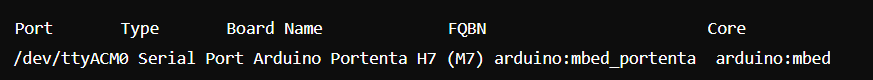
\includegraphics[width=0.7\linewidth]{Images/ArduinoCLI/CLIBoardList.png}
		\caption{ Return values of the “board list” function }
		\label{CLIBoardList}
	\end{center}
\end{figure}

\subsection{Configuration of Arduino CLI}

To begin with, the correct core for the Arduino Portenta H7 should be installed. Before that, add the staging index URL to the Arduino CLI configuration file \FILE{arduino-cli.yaml} with the following command \SHELL{arduino-cli config add board\_manager.additional\_urls \\https://downloads.arduino.cc/packages/package\_staging\_\\index.json}. Then update the board index to fetch the latest package information from the staging index using the command \SHELL{arduino-cli core update-index} as shown in the Figure ~\ref{CoreIndex}.
\begin{figure}
	\begin{center}
		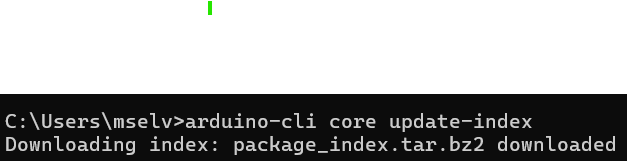
\includegraphics[width=0.7\linewidth]{Images/ArduinoCLI/CoreIndex.png}
		\caption{Updating the board index}
		\label{CoreIndex}
	\end{center}
\end{figure}
\begin{figure}
	\begin{center}
		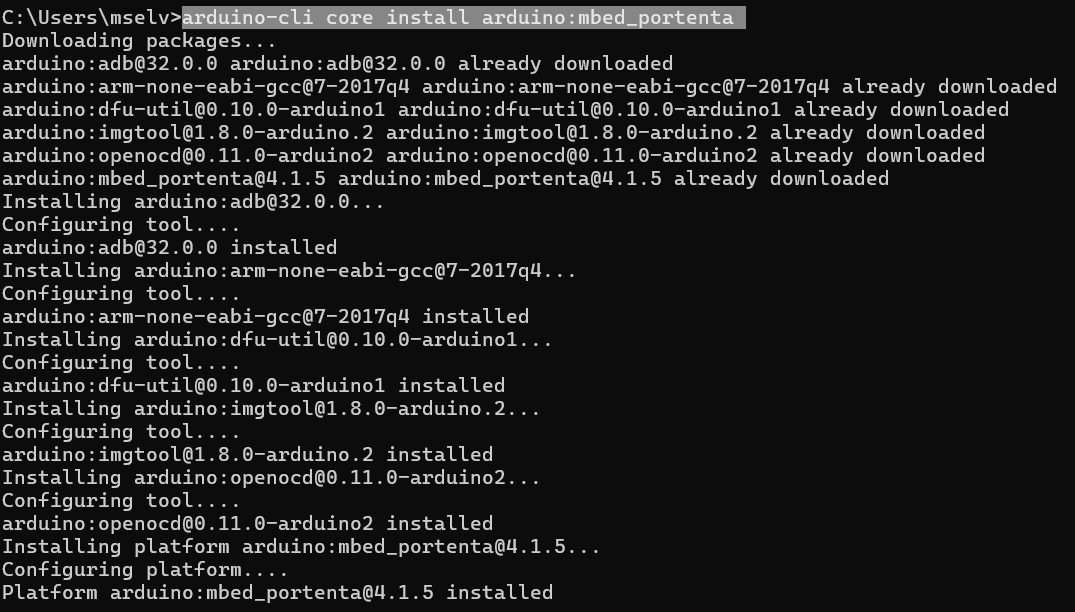
\includegraphics[width=0.7\linewidth]{Images/ArduinoCLI/CoreInstall.png}
		\caption{Installing the core for Arduino Portenta H7}
		\label{CoreInstall}
	\end{center}
\end{figure}

Once the index is updated, install the Portenta H7 boards core that are available in the staging index using the command \SHELL{arduino-cli core install arduino:mbed\_portenta} as shown in the Figure ~\ref{CoreInstall} and the correct core name "arduino:mbed" can be fetched from the Figure ~\ref{CLIBoardList}.
\begin{figure}
	\begin{center}
		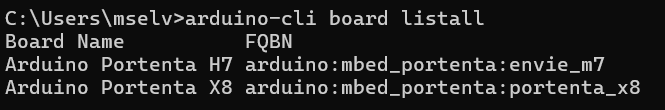
\includegraphics[width=0.7\linewidth]{Images/ArduinoCLI/Listall.png}
		\caption{List available boards}
		\label{Listall}
	\end{center}
\end{figure}

Now run the command \SHELL{arduino-cli board listall} to view all boards supported by the installed cores as shown in the Figure ~\ref{Listall}

\subsection{Creating a new sketch}
The first step is to create a new sketch:

\SHELL{arduino-cli sketch new cli\_test}
	
This command creates a directory named \FILE{cli\_test}, which contains a file with the same name as shown in the Figure ~\ref{NewSketch}
\begin{figure}
	\begin{center}
		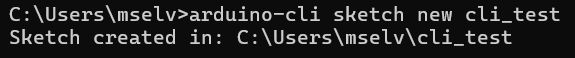
\includegraphics[width=0.7\linewidth]{Images/ArduinoCLI/NewSketch.png}
		\caption{Creating a new Sketch with CLI}
		\label{NewSketch}
	\end{center}
\end{figure}

\subsection{Compiling a sketch}
The function \SHELL{compile} of CLI can be used to compile a sketch for any supported board. The crucial option required by this function is the board type, which can be specified with the option \SHELL{--fqbn}. The abbreviation \SHELL{fqbn} means "fully-qualified board name". For example, the following boards are available:
\begin{itemize}
	\item Arduino Uno: \SHELL{arduino:avr:uno}
	\item Arduino Mega: \SHELL{arduino:avr:mega}
	\item Arduino Micro: \SHELL{arduino:avr:micro} 
	\item Arduino Mini: \SHELL{arduino:avr:mini}
	\item Arduino Portenta H7: \SHELL{arduino:mbed\_portenta}
	\item Arduino Portenta X8 : \SHELL{arduino:mbed\_portenta:portenta\_x8}
	\item ESP32 Dev Module: \SHELL{esp32:esp32}
\end{itemize}

The possible boards are structured as follows: \\
\SHELL{manufacturer:architecture:board}.

With the following command, the example sketch, which is located in the folder \FILE{C:/Users/user.name} can be compiled for an Arduino Portenta H7: 
\SHELL{arduino-cli compile --fqbn arduino:mbed\_portenta:envie\_m7 C:/Users/mselv/cli\_test}
%\medskip
\newline
\begin{figure}
	\begin{center}
		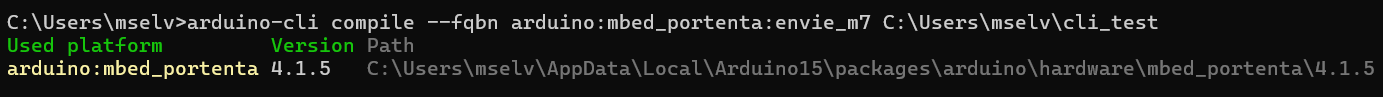
\includegraphics[width=0.7\linewidth]{Images/ArduinoCLI/CompileSketch.png}
		\caption{Compiling a sketch with CLI }
		\label{CompileSketchCommand}
	\end{center}
\end{figure}
Figure ~\ref{CompileSketchCommand} shows the CLI messages. The following flags can be added:
\begin{itemize}
	\item Verbose \SHELL{-v}: Useful if you want to display all options and files that are compiled in your sketch.
	\item Build path \SHELL{--build-path [string]}: Useful if the compiled object and hex files are to be saved in a custom path. On my Windows system, the value of this parameter must be a complete path.
\end{itemize}

\subsection{Uploading a sketch}
A compiled sketch can be uploaded. Similar to the compile command, the upload command also requires the use of the option \SHELL{-fqbn}. Additionally, a serial interface is necessary for uploading, which is specified with the option \SHELL{-p}. The following command uploads the example sketch to a Windows COM port on COM18 as shown in Figure ~\ref{UploadSketchCLI}:

	\SHELL{arduino-cli upload -p COM18 --fqbn arduino:mbed\_portenta:envie\_m7 C:/Users/mselv/cli\_test}


If executed correctly, the RX/TX LEDs of the Arduino should start flashing, and shortly afterward, an empty sketch will be executed.

\subsection{Installation of Libraries}
If a library is required, you can first use the command

	\SHELL{arduino-cli lib search ethernet}

to check if the library (in this case, Ethernet) is installed. Then, with the command

	\SHELL{arduino-cli lib install "UIPEthernet"}
	
you can install it.

\subsection{Example program "Hello World"}
The "Hello World!" counterpart for microcontrollers will be used to demonstrate how to compile a sketch and then upload it using the Arduino CLI. A simple sketch that makes the Arduino's LED flash is used for this.

\begin{code}
% Include a specific range of lines from the C++ file
\lstinputlisting[language=C++, firstline=1, lastline=81, label={lst:arduinoBlink}]{../Code/Arduino/ArduinoCLI/BLINK.ino}
\end{code}

In the function \SHELL{setup()}, which is executed once at the beginning, the built-in LED is defined as an output \SHELL{pinMode(LED\_BUILTIN, OUTPUT)}. This allows the LED to be controlled later. Within the \SHELL{loop()} function, the LED is first switched on \SHELL{digitalWrite(LED\_BUILTIN, HIGH)} and then switched off again with a delay of one second \SHELL{delay(1000)}. Before the LED is switched on again at the beginning of the loop, another second is waited at the end of the loop to achieve the flashing effect.

To compile the sketch, the command previously defined as the basic function \SHELL{compile}, as shown in Figure \ref{CompileSketchCommand}, can be used.

The compiled sketch can then be uploaded to the Arduino Portenta H7 using the function \SHELL{upload} as shown in Figure ~\ref{UploadSketchCLI}

\begin{figure}
	\begin{center}
		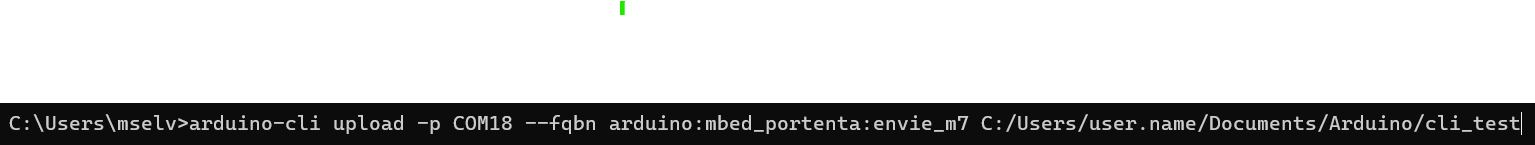
\includegraphics[width=0.7\linewidth]{Images/ArduinoCLI/UploadSketch.png}
		\caption{Uploading the compiled sketch}
		\label{UploadSketchCLI}
	\end{center}
\end{figure}

After the successful upload, the LED of the Arduino Portenta H7 shown in Figure \ref{LEDflash} starts to flash.
\begin{figure}
	\begin{center}
		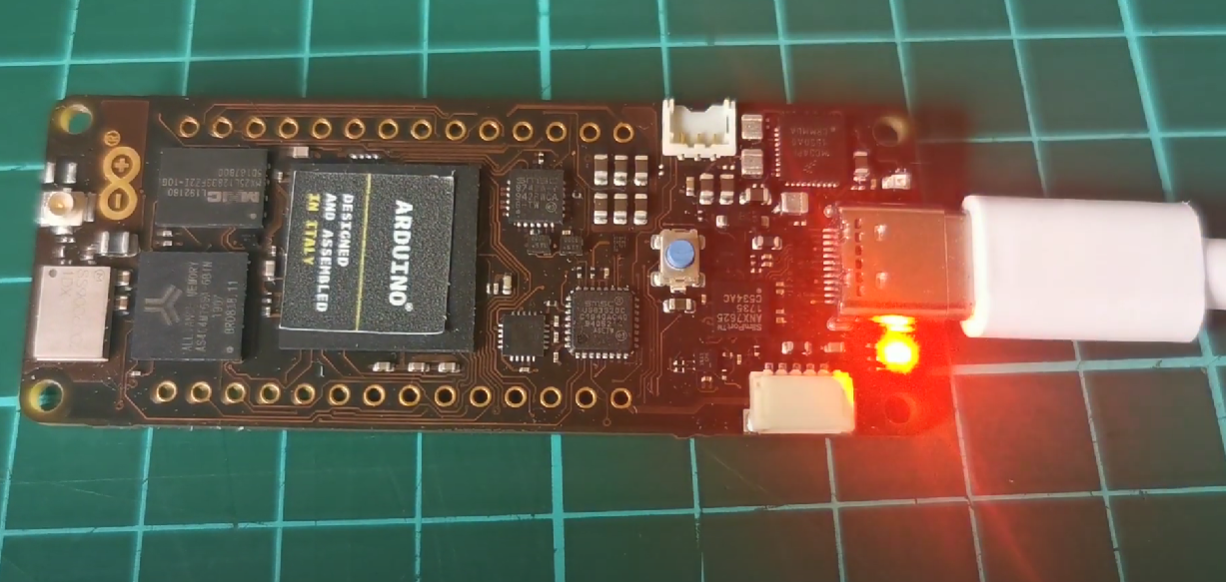
\includegraphics[width=0.7\linewidth]{Images/ArduinoCLI/Blink.png}
		\caption{The orange LED of the Arduino starts to flash}
		\label{LEDflash}
	\end{center}
\end{figure}

\chapter{Batch File}

\section{Batch File}

A batch file is a text file that contains a sequence of commands intended to be executed by the command-line interpreter. On Windows operating systems, these files typically have the extension \FILE{.bat} or \FILE{.cmd}. Batch files are used to automate repetitive tasks, perform complex sequences of commands, and streamline system administration processes. The results are documented in a log file.  \cite{microsoftWindowsCommands:2025}

\section{List Batch File}
A "list batch file" refers to a batch file designed to list specific items, such as files in a directory, the contents of a directory, or any other listable resources. In the context of Arduino CLI, a list batch file might include commands to list available Arduino boards, libraries, or sketches.

\begin{center}
	\begin{lstlisting}
@echo off
:: List available Arduino boards
arduino-cli board list
	\end{lstlisting}
\end{center}

\SHELL{@echo off} command is used at the beginning of the batch file to suppress the display of each command as it executes. By default, batch files echo each command to the console as they execute, but \SHELL{@echo off} prevents this behavior, making the output cleaner. 
\SHELL{:: List available Arduino boards} is a comment in the batch file. In batch scripting, comments start with :: or rem, and they are ignored by the command interpreter.
\SHELL{arduino-cli board list} command executes the arduino-cli command-line tool with the board list subcommand. This subcommand lists all available Arduino boards connected to the system

\section{Explanation of Batch commands}

This section describes how the batch script works.

{\small 
\begin{lstlisting}
@echo off
echo log file Arduino setup, %time% clock, %date% > setup-log.txt
echo. >> setup-log.txt
echo. >> setup-log.txt
\end{lstlisting}
}

The command \SHELL{\@echo off} prevents the script content from being output during execution. This enables more appealing front-end programming. The log file is created in the second line. When it is created, the first line of the log is given the heading \SHELL{Logfile Arduino setup} and the system time \SHELL{\%time\%} and date \SHELL{\%date\%} are read out. For later clarity of the log file, two empty lines \SHELL{echo. >> setup-log.txt}. If the greater than operator \SHELL{> setup-log.txt} is used once, a new file is created or an existing file with the same name is overwritten. If the greater than operator \SHELL{>> setup-log.txt} is used twice, the left-hand content is appended to an existing file in a new line. In this way, the log file is written line by line and not once completely at the end of the batch script.

\begin{center}
\begin{lstlisting}
	:: If necessary, the core is installed
	echo core status: >> setup-log.txt
	arduino-cli core install arduino:mbed_portenta >> setup-log.txt
\end{lstlisting}
\end{center}

Comments in the batch script are identified by two consecutive colons \SHELL{:: If necessary, the core is installed} and are intended to increase traceability within the script. The command \SHELL{echo core status: >> setup-log.txt} is used in the log file to indicate that the next line contains information about the core to be installed for the Arduino Portenta H7. The Arduino CLI already has the intelligence to check whether the specified core is already installed. If this is the case, the corresponding documentation is included in the log file. The installation of the core is initialized with the line \SHELL{arduino-cli core install arduino:mbed\_portenta >> setup-log.txt}. The core required for the Arduino Portenta H7 is specified with the name \SHELL{arduino:mbed\_portenta}. The return value of the function for core installation is saved in the log file.

\begin{lstlisting}
echo A search is made for connected boards...
:: List the connected Arduinos
echo The following boards are connected to the PC: >> setup-log.txt
echo.
echo. >> setup-log.txt
arduino-cli board list >> setup-log.txt
arduino-cli board list
echo.
\end{lstlisting}
At the beginning of this script section, the user of the software is first informed about the search for the connected Arduino boards \SHELL{echo A search for connected boards is performed...}. The following command \SHELL{echo The following boards are connected to the PC: >> setup-log.txt} informs the user about the content of the next line in the log file. Information about which Arduinos are connected to the PC can be obtained with the command \SHELL{arduino-cli board list}, which is executed twice here. In the first execution, the return of the Arduino-CLI is saved in the log file \SHELL{>> setup-log.txt}, the second execution is used for display in the currently executed script. The user needs the information about the connected Arduinos for an input in the next step.

\begin{lstlisting}
:: Query the port name for later upload 
:: of the sensor test file
set /p port="Please enter the port name of the Portenta H7 and confirm: "
echo The port %port% was selected. >> setup-log.txt
\end{lstlisting}

In the line \SHELL{set /p port="Please enter the port name of the Portenta H7 and confirm:"} a user query is displayed. The command \SHELL{set} allows the variable \SHELL{port} to be set to a specific value. With the addition \SHELL{/p}, this specific value is set to the following user input. Execution of the script is stopped until the user input is successful. The user input contains the port of the connected Arduino Nano 33 BLE Sense Lite. For later traceability, the selected port is entered in the log file with the line \SHELL{echo The port \%port\% was selected. >> setup-log.txt} is documented. 

\begin{lstlisting}
:: Create the folder for the compiled sensor test
set folder=SensorTestCompiledData
mkdir %folder%
\end{lstlisting}

The variable \SHELL{folder} is assigned the value \SHELL{SensorentestCompiledData}. In the next line \SHELL{mkdir \%folder\%} the folder with the name \PYTHON{SensorentestCompiledData} is created for saving the compiled sketch later.

\begin{lstlisting}
:: If necessary, the required libraries for 
:: the sensor test are installed

:: Library for the onboard LPS22HB barometer
echo Lib for LPS22HB barometer >> setup-log.txt
arduino-cli lib install Arduino_LPS22HB >> setup-log.txt
echo. >> setup-log.txt

:: Library for the onboard HTS221 temperature and humidity sensor
echo Lib for HTS221 temperature and humidity sensor >> setup-log.txt
arduino-cli lib install Arduino_HTS221 >> setup-log.txt
echo. >> setup-log.txt
\end{lstlisting}

The log file documents which library is involved in the following line \SHELL{SensorentestCompiledData}. Then use the command \SHELL{arduino-cli lib install Arduino\_LPS22HB >> setup-log.txt} to install the library and save the return value of the installation in the log file. A library that has already been installed is recognized by the Arduino CLI and a corresponding return value is written to the log file. The procedure is identical for all three libraries to be installed.

\begin{lstlisting}
:: Compiling the sensor test sketch
echo Compiling the sensor test sketch: >> setup-log.txt
echo. >> setup-log.txt
arduino-cli compile -b arduino:mbed_portenta:envie_m7 
%cd%\SensortestPortentaH7 
--build-path %cd%\%folder% >> setup-log.txt
\end{lstlisting}

Once the necessary libraries have been installed, the previously created sketch for testing the sensors can be compiled. The sketch for the Arduino Nano 33 BLE Sense Lite is compiled with the command \SHELL{arduino-cli compile -b arduino:mbed\_portenta:envie\_m7 \%cd\%/SensortestPortentaH7}. The last part of the command specifies the memory path of the sketch to be compiled. Furthermore, the target folder for the compiled sketch can be defined with the addition \SHELL{--build-path \%cd\%/\%folder\% >> setup-log.txt}. The return value of compiling with the Arduino CLI is saved in the log file.

\begin{lstlisting}
:: Upload the compiled sketch to the Arduino
echo Upload the compiled sketch to the Arduino >> setup-log.txt
arduino-cli upload -p %port% --input-dir %cd%\%folder% 
>> setup-log.txt
\end{lstlisting}

The compiled sketch is stored in the line \SHELL{arduino-cli upload -p \%port\% --input-dir}  \SHELL{\%cd\%/\%folder\% >> setup-log.txt} to the Arduino Portenta H7 connected via \SHELL{port}. The storage path of the compiled data is specified with the addition \SHELL{--input-dir \%cd\%/\%folder\%}.

\begin{lstlisting}
:: Opening the serial monitor
start monitor_log
:: Automatic closing of the serial monitor after 4 seconds 
:: (n-1 seconds, with n=5)
ping 127.0.0.1 -n 5 > nul
taskkill /im serial-monitor.exe /F
\end{lstlisting}

The command \SHELL{start monitor\_log} calls another batch script to read out the serial monitor. The line \SHELL{ping 127.0.0.1 -n 5 > nul} stops the execution of the software for four seconds. Five requests are sent to the local computer and one second is waited between each request. With \SHELL{> nul}, the output of the responses is directed to the void and not displayed. Once the four-second period has elapsed, the serial monitor for reading the sensor data is automatically closed with the command \SHELL{taskkill /im serial-monitor.exe /F}. The window to be closed can be named \SHELL{serial-monitor.exe} using the suffix \SHELL{/im}. The forced closing of the serial monitor takes place with the appendix \SHELL{/F}. After the serial monitor has been read out and closed, the software can be closed. The results of the sensor test can then be found in the log file.

The serial monitor is opened in the script \FILE{monitor\_log.bat}.

\begin{lstlisting}
echo Sensor data: >> setup-log.txt
echo. >> setup-log.txt

echo The serial monitor is opened, the sensor data is 
read out and saved in the log file...

arduino-cli monitor -p %port% >> setup-log.txt
\end{lstlisting}	

The serial monitor can be activated using the Arduino CLI command \SHELL{arduino-cli monitor} \SHELL{-p \%port\% >> setup-log.txt} to open it. The connection for the specified port is established with \SHELL{-p \%port\%}. With the addition \SHELL{>> setup-log.txt} the received data is written to the log file.
